\chapter{Pseudokód - Výpočet statistik}
\begin{algorithm}
\caption{Výpočet statistik}
\label{alg:computeStat}
	\begin{algorithmic}[1] \STATE{\textbf{funkce}
vypočtiStatistiky (poleBody)} \STATE{kumulativníČas = 0}
\STATE{časSegmentPředchozí = 0} \STATE{časMimoRastr = 0}
\STATE{délkaMimoRastr = 0} \STATE{početBodůRastr = 0}
\STATE{kumulativníDávka = 0} \STATE{hodnotaRastrPředchozí = 0}
\STATE{průměrnýPříkon = 0} \STATE{délkaTrasy = 0}
\STATE{maximálníPříkon = 0}

		\FOR{i = řada od 0 do délka(poleBody)} \IF{i <
délka(poleBody) - 1} \STATE{vzdálenost =
vypočtiVzdálenost(poleBody[i], poleBody[i+1])} \ELSE \STATE{vzdálenost
= 0}
			\ENDIF
			
			\STATE{délkaTrasy = délkaTrasy + vzdálenost}

			\STATE{časSegment = vzdálenost / rychlost}
\STATE{kumulativníČas = kumulativníČas + časSegmentPředchozí}
\STATE{dávkaSegment = časSegmentPředchozí $\cdot$
hodnotaRastrPředchozí} \STATE{kumulativníDávka = kumulativníDávka +
dávkaSegment} \STATE{hodnotaRastr = získejHodnotu(poleBody[i])}

		\algstore{myalg}
		\end{algorithmic}
		\end{algorithm}

		\begin{algorithm}
		\begin{algorithmic} [1] \algrestore{myalg}

			\IF{bod1 mimo rastr \textbf{or} hodnotaRastr
<= 0} \STATE{hodnotaRastr = 0} \STATE{časMimoRastr = časMimoRastr +
časSegment} \STATE{délkaMimoRastr = délkaMimoRastr + vzdálenost} \ELSE
\STATE{průměrnýPříkon = průměrnýPříkon + hodnotaRastr}
\STATE{početBodůRastr = početBodůRastr + 1}
			\ENDIF
			
			\IF{hodnotaRastr > maximálníPříkon}
\STATE{maximálníPříkon = hodnotaRastr}
			\ENDIF \STATE{přidej [hodnotaRastr,
kumulativníČas, časSegmentPředchozí, kumulativníDávka] do
poleAtributů} \STATE{hodnotaRastrPředchozí = hodnotaRastr}
\STATE{časSegmentPředchozí = časSegment}
		\ENDFOR
		
		\STATE{průměrnýPříkon = průměrnýPříkon /
početBodůRastr} \STATE{statistiky = [délkaTrasy, kumulativníČas,
délkaMimoRastr, časMimoRastr, maximálníPříkon, průměrnýPříkon,
kumulativníDávka]} \STATE{\textbf{return} poleAtributů, statistiky}
	\end{algorithmic}
\end{algorithm}


\chapter{User guide} \label{User guide}
This plugin computes the gamma radiation dose of a given route on an
interpolated map of dose rate values. The secondary product of the
plugin are basic statistics about the given route. Together, these
output values help the emergency teams to determine which route will be
the best and safest for mobile radiation monitoring teams for radiation
monitoring during nuclear disaster emergency exercises (or~during the
nuclear disaster itself). It is important to mention, that results of~the~computation, especially
those, that~are~dealing with~the~gamma radiation dose, are~estimates.
The reason of this is, that the calculations only use few of~variables,
that are dealing with this problematics. For example it does not concern
the~situation on roads, weather (wind, rain..) etc.

\section{Installation}
Best way to install the plugin is via QGIS plugin repository.
Follow these instructions:

\begin{enumerate}
\item
  Go to \texttt{Plugins} drop down menu and select
  \texttt{Manage and Install Plugins...}:


\begin{figure}[H]
\centering
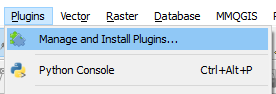
\includegraphics{pictures/user_guide/install_plugin_dropdown.png}
\caption{Plugins menu.}
\end{figure}

\item At this time, this plugin is not registered in the official QGIS
repository, therefore it is required to add its home repository CTU
GeoForAll Lab for it to be visible in~the~list of plugins. In order to
this to be done, in \texttt{Settings} tab hit \texttt{Add...} button and
type \url{http://geo.fsv.cvut.cz/geoforall/qgis-plugins.xml} to~\texttt{URL} 
slot.

\textbf{Note: }It is also required to tick \texttt{Show also experimental plugins} 
since this plugin is distributed as experimental. In future, the plugin 
will be published in~the~official QGIS repository.


\begin{figure}[H]
\centering
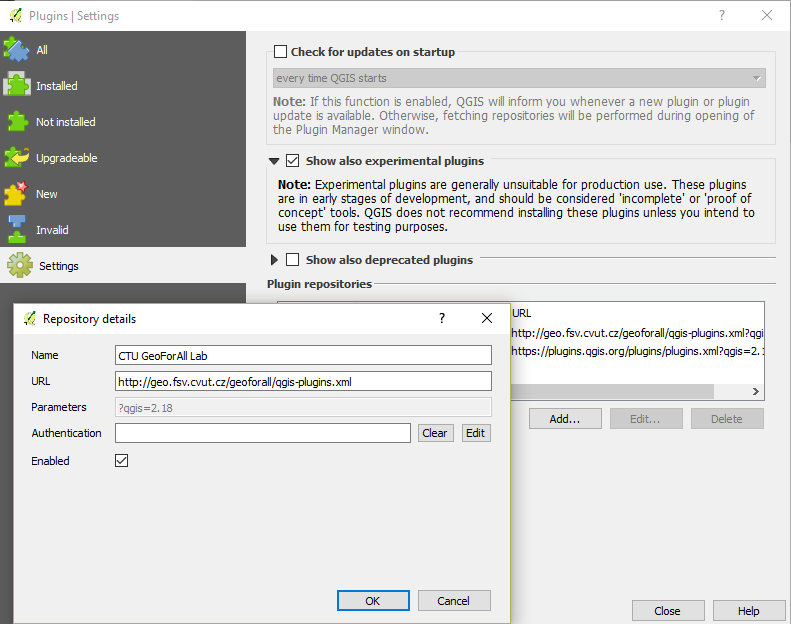
\includegraphics[scale = 0.7]{pictures/user_guide/settings.png}
\caption{Add home repository of the plugin.}
\end{figure}



\item 
Search for \texttt{Ground\ Radiation\ Monitoring} plugin on the
\texttt{All} or \texttt{Not\ installed} tab. After selecting the plugin,
hit \texttt{Install\ plugin} button:

\begin{figure}[H]
\centering
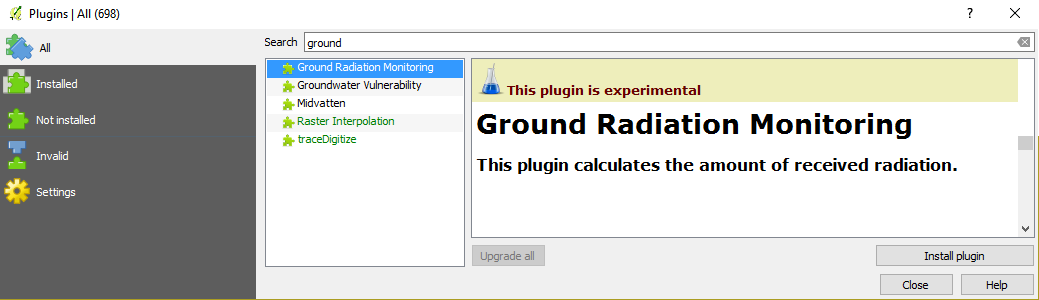
\includegraphics[scale=0.55]{pictures/user_guide/install_search_plugin.png}
\caption{Search and install the plugin.}
\end{figure}

\item
The Ground Radiation Monitoring Plugin is ready to use with the icon
appearance in the QGIS toolbar:

\begin{figure}[H]
\centering
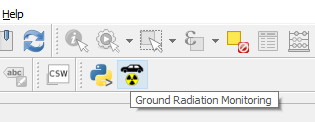
\includegraphics{pictures/user_guide/install_toolbar.png}
\caption{Ground Radiation Monitoring Plugin on the QGIS toolbar.}
\end{figure}

\end{enumerate}

\section{Plugin description}

\subsection{Sampling the track}\label{sampling-the-track}

The distance between track vertices can be very large, especially on
sections, that are straight (e.g. highways). If there is any kind of
peak or any significant change of dose rate value on these long straight
parts of track, it is not recognized because of the stated reason. Hence
the plugin samples the track to smaller parts and allows user to choose
the length of them.

\subsection{GUI}\label{gui}

The plugin is divided into two tabs. The first of them is \texttt{Main}
tab:

\begin{figure}[H]
\centering
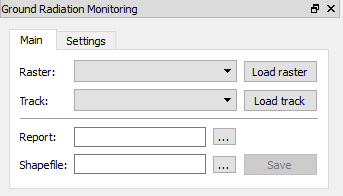
\includegraphics{pictures/user_guide/gui_main.png}
\caption{The main tab of plugin.}
\end{figure}

\begin{itemize}

\item
  In main tab, the user may select a raster layer with the interpolated
  map of dose rate values. He may select a vector layer with a route.
  Both of those layer could be selected using combo boxes, which include
  available layers from the Layer panel. There is a restriction for the
  track combo box, that only the layer with a linestring type is being
  shown.
\item
  Plugin also allows user to upload files with raster and vector layers
  via buttons \texttt{Load\ raster} and \texttt{Load\ track}. With
  hitting one of these buttons, a file dialog appears. Only GDAL/OGR
  supported files are shown.
\item
  A tool button \texttt{...} that follows \texttt{Report} line lets the
  user to select a destination, where the report file will be saved.
  Then the blank space in the same line is filled with the path to
  selected destination file with \emph{.txt} suffix. Also the blank
  space in~the~\texttt{Shapefile} is automatically filled with the same
  path with a different suffix (\emph{.shp} instead of \emph{.txt}).
\item
  The destination of the created shapefile could be changed with hitting
  a tool button \texttt{...} on \texttt{Shapefile} line.
\item
  Finally, \texttt{Save} button does all the work, it starts the
  computation and saves created files to selected destinations.
\end{itemize}

The second tab of the plugin is \texttt{Settings} tab:

\begin{figure}[H]
\centering
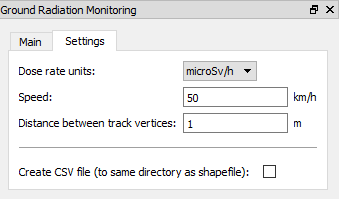
\includegraphics{pictures/user_guide/gui_settings.png}
\caption{The settings tab.}
\end{figure}

\begin{itemize}
\item
  This tab allows the user to change input variables.

  \begin{itemize}
  
  \item
    \texttt{Dose\ rate\ units} combo box sets the units of gamma
    radiation dose rate values of the interpolated map.
  \item
    \texttt{Speed} value determines what speed the mobile team is
    driving. This value has to be given.
  \item
    \texttt{Distance\ between\ track\ vertices} value is used for
    sampling the track. If~this value is not given, the track will not
    be sampled.
  \item
    \texttt{Create\ CSV\ file} checkbox gives the user an option,
    whether to create CSV file with the same data, that are written to
    created shapefile.
  \end{itemize}
\item
  Settings tab is filled with values by default.
\end{itemize}

\subsection{Input data}\label{input-data}

\begin{figure}[H]
\centering
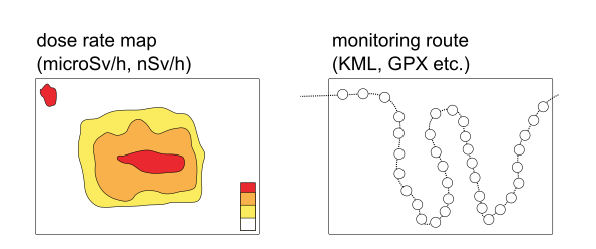
\includegraphics{pictures/user_guide/input.png}
\caption{Input files.}
\end{figure}

\begin{itemize}

\item
  An interpolated map of dose rate values with a format supported by
  \href{http://www.gdal.org/formats_list.html}{GDAL library}.
\item
  A monitoring linestring route with a format supported by
  \href{http://www.gdal.org/ogr_formats.html}{OGR library}.
\end{itemize}

\subsection{Output data}\label{output-data}

\begin{itemize}

\item
  A text report file containing fields:

  \begin{itemize}
  \item
    time, when was the report created;
  \item
    route information - name, monitoring speed, total monitoring time,
    total distance;
  \item
    information about the part of the track, that has no data available
    (where the~track exceeds the raster) - time, distance;
  \item
    estimated radiation values - maximum and average dose rate, total
    dose;
  \item
    plugin settings - input raster units, distance between track
    vertices.
  \item
    a static text explaining the report
  \end{itemize}
\end{itemize}

\begin{figure}[H]
\centering
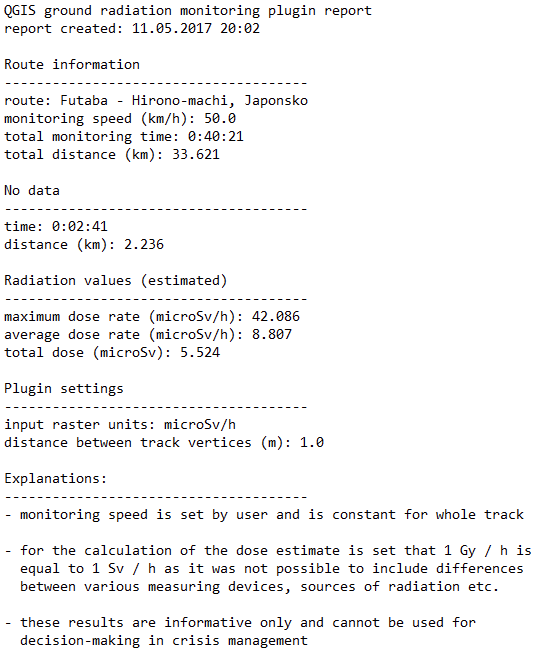
\includegraphics{pictures/user_guide/report.png}
\caption{The report file.}
\end{figure}

\begin{itemize}

\item
  A shapefile with point layer counting vertices of a sampled route with
  following attributes - dose rate, cumulated time, time interval from
  previous point, cumulated dose.
\end{itemize}

\begin{figure}[H]
\centering
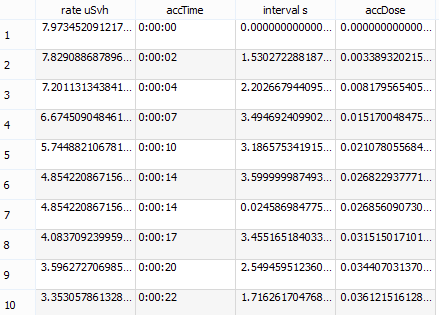
\includegraphics{pictures/user_guide/shapefile.png}
\caption{The attribute table.}
\end{figure}

\begin{itemize}
\item
  An optional CSV file with same values as in created shapefile.
\end{itemize}

\begin{figure}[H]
\centering
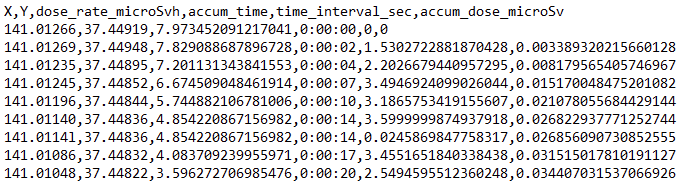
\includegraphics[scale = 0.8]{pictures/user_guide/csv.png}
\caption{The CSV file.}
\end{figure}



